% ---------------------------------------------------------------------------
\section{Evaluation}
\label{sec:evaluation}

\paragraph{Protocol} Version~21 was run with 24 keys on the same text (the opening of Isidore's \emph{Etymologiae}
XVII, 38{,}304 bits). Keys 1--12 had also been used during development to choose between variants; keys 13--24 never
were. Each book was judged by the two judges, the scorecard, the eight extra properties and the line gate, read back with
its key and with a wrong key.

\begin{table}[htbp]
\centering\footnotesize
\caption{Version~21 on 24 keys: the instruments of Section~\ref{sec:scorecard} (mean $\pm$ standard error over keys).
Lower part: each scorecard property, Voynich value, mean of the generated books, and the number of keys whose book fails
it.}
\label{tab:results}
\begin{tabularx}{\linewidth}{Yrrr}
\toprule
 & keys 1--12 & keys 13--24 (fresh) & all 24 \\
\midrule
AUC judge 1 & $0.554 \pm 0.006$ & $0.554 \pm 0.005$ & $0.554 \pm 0.004$ (0.517--0.580) \\
AUC judge 2 & $0.596 \pm 0.008$ & $0.606 \pm 0.006$ & $0.601 \pm 0.005$ (0.551--0.632) \\
keys with judge 2 above 0.60 & 6 & 8 & 14 \\
scorecard (of 17 attainable) & 16.0 & 15.9 & 16.0 \\
extra properties (of 8) & 5.5 & 5.2 & 5.4 \\
line gate passed & 12 of 12 & 12 of 12 & 24 of 24 \\
exact read-back; wrong key rejected & 12; 12 & 12; 12 & 24; 24 \\
capacity (bits) & & & 81{,}100--85{,}900 \\
\bottomrule
\end{tabularx}

\vspace{0.6em}
\begin{tabularx}{\linewidth}{rYrrr}
\toprule
\# & scorecard property & Voynich & generated (mean) & keys failing \\
\midrule
1 & $h_2$ & 2.236 & 2.284 & 0 \\
2 & predictability of the space & 0.664 & 0.639 & 0 \\
3 & words occurring once & 0.678 & 0.738 & 0 \\
4 & types per token & 0.210 & 0.205 & 0 \\
5 & identical neighbours relative to the line & 1.009 & 0.943 & 0 \\
6 & homogeneity within the line & 0.0385 & 0.0414 & 1 \\
7 & gradient (not attainable) & 0.683 & 0.62 & 24 \\
8 & junction & 0.188 & 0.180 & 0 \\
9 & attested joins relative to chance & 1.97 & 2.13 & 0 \\
10 & flat curve of once-occurring words & 0.057 & $-0.024$ & 0 \\
11 & vocabulary turnover & 0.106 & 0.095 & 0 \\
12 & page profile (ratio) & 1.06 & 0.66 & 24 \\
13 & autocorrelation of word lengths & 0.150 & 0.142 & 0 \\
14 & Zipf slope & $-1.041$ & $-1.005$ & 0 \\
15 & word shape & 0 & 0.040 & 0 \\
16 & vertical similarity & 1.028 & 1.035 & 0 \\
17 & formulas & 6.39 & 4.58 & 0 \\
18 & line edges (start; end) & 23; 55 & 23.6; 54.5 & 0 \\
\bottomrule
\end{tabularx}
\end{table}

\begin{figure}[htbp]
\centering
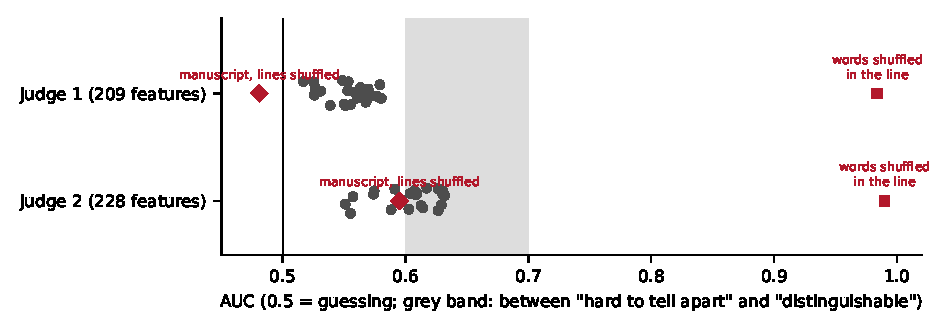
\includegraphics[width=\linewidth]{figure/valutazione.pdf}
\caption{AUC of the two judges for the books of the 24 keys (dots), against the real manuscript degraded on purpose
(red): with its lines shuffled within each page, and with its words shuffled within each line. Data:
\expcode{e409b} (version~21) and \expcode{e400}.}
\label{fig:evaluation}
\end{figure}

\paragraph{How close to the manuscript} The first judge separates generated from real pages with AUC 0.55, the second
with 0.60 (Table~\ref{tab:results}, Figure~\ref{fig:evaluation}); on the fresh keys the second judge gives 0.606. For the
second judge this is the level of the real manuscript with its lines shuffled within each page (0.595), and far from
the manuscript with its words shuffled within each line (0.99). The group of features that the second judge uses best
is the register of the first lines of paragraphs (AUC 0.62 on that group alone). The books pass 16 of the 17
attainable scorecard properties: they always miss the page profile, a measure of how much each page departs from its
section, and once the homogeneity within the line. Of the extra properties they usually miss the spelling choices that
vary from line to line (23 of 24 keys), the register of the first lines (18 of 24) and the spread of word lengths (20 of
24). Lines are too irregular in width: 11.6\% are wider than 1.25 times the page median, against 6.0\% in the
manuscript. About 0.4--0.5\% of the word triples of a book also occur in the manuscript.

\paragraph{With and without a message} [e419: with 24 keys, books with the Isidore text and books with filler only;
differences of the two judges against the manuscript, and a direct classifier between the two kinds of book.]

\paragraph{What the generator does not do} It writes only running paragraph text: no labels, no circular or radial
text, and no images (the website places the real drawings next to the generated folios). It does not model hands, and
it generates pages independently, so the bifolium effects of Section~\ref{sec:book} are absent. It models copying from
the line above by the index of the word in the line, whereas the manuscript copies by physical position. Two rules of
Section~\ref{sec:rules} that are not in the instruments, the closure at the gap of a drawing and the drift along the
line, were not targeted, and the short state only as agreement of the spelling choices within a line.
